\documentclass[12pt,spanish]{homework}
\usepackage[utf8]{inputenc}
\usepackage[T1]{fontenc}
%\usepackage{mathpazo}
\usepackage{graphicx}
\usepackage{booktabs}
\usepackage{listings}
\usepackage{enumerate} 
\usepackage{amsmath}
\usepackage{amssymb}
\usepackage[spanish,mexico]{babel}
\inputencoding{latin1}

\title{Variables Uniformes Discretas}
\author{Emilio Balan,Amilcar Campos, Elian Carrasco, Citlali Guti�rrez, H�ctor Rodr�guez}
\date{4 de noviembre del 2020}
\institute{Universidad Aut�noma de Yucat�n \\ Facultad de Matem�ticas - UADY}
\class{Probabilidad 1 (Grupo B)}
\professor{Lic. Ernesto Guerrero Lara}

\begin{document}

\maketitle

\section*{Experimento que origina a la variable uniforme discreta}
Es la distribuci�n de probabilidad se asocia a variables cuyos posibles valores tienen todos la misma probabilidad. Si una variable aleatoria X cuyos posibles valores son $({x_{1}, . . . ,x_{n}})$  
tiene distribuci�n uniforme discreta entonces
$$
P(X=x_{1})=P(X=x_{2})=...=P(X=x_{n})={\dfrac{1}{n}}
$$
Decimos que una variable aleatoria X tiene una distribuci�n uniforme discreta sobre el conjunto de n n�meros $\lbrace x_{1}, . . . , x_{n} \rbrace$ si la probabilidad de que
X tome cualquiera de estos valores es constante $\dfrac{1}{n}$. Esta distribuci�n surge
en espacios de probabilidad equiprobables, esto es, en situaciones en donde
tenemos n resultados diferentes y todos ellos tienen la misma probabilidad
de ocurrir.
Los juegos de loter�a son un ejemplo donde puede aplicarse esta distribuci�on de probabilidad.
Se denota c�mo $X \sim$ unif$\lbrace x_{1}, . . ., x_{n} \rbrace$, en donde el s�mbolo $\sim$ se lee "se distribuye como" o "tiene una distribuci�n". 
\section*{Funci�n masa de probabilidad de la variable}
La funci�n de probabilidad de esta variable aleatoria es:
$$
f_{X} (x)=\begin{cases}
{\dfrac{1}{n}} & si \mbox{ $x=x_{1},...,x_{n}$}\\{0 }& \mbox{otro caso}\
\end{cases}
$$
La gr�fica de la funci�n de probabilidad de la distribuci�n uniforme en el conjunto (1,2,3,4,5) aparece en la figura siguiente, junto con la correspondiente funci�n de distribuci�n. Cada salto en la funci�n de distribuci�n es de tama�o $\dfrac{1}{5}$. La expresi�n completa de $F_{X}(x)$ es la siguiente:
$$
F_{X} (x)=\begin{cases}
\ {0} &  \mbox{ $x<1$}\\ {0.20} &  \mbox{ $1\leq x<2$}\\ {0.40} &  \mbox{ $2\leq x<3$}\\ {0.60} &  \mbox{ $3\leq x<4$}\\ {0.80} &  \mbox{ $4\leq x<5$}\\ {1} &  \mbox{$ x\geq 5$}\
\end{cases}
$$
\begin{center}
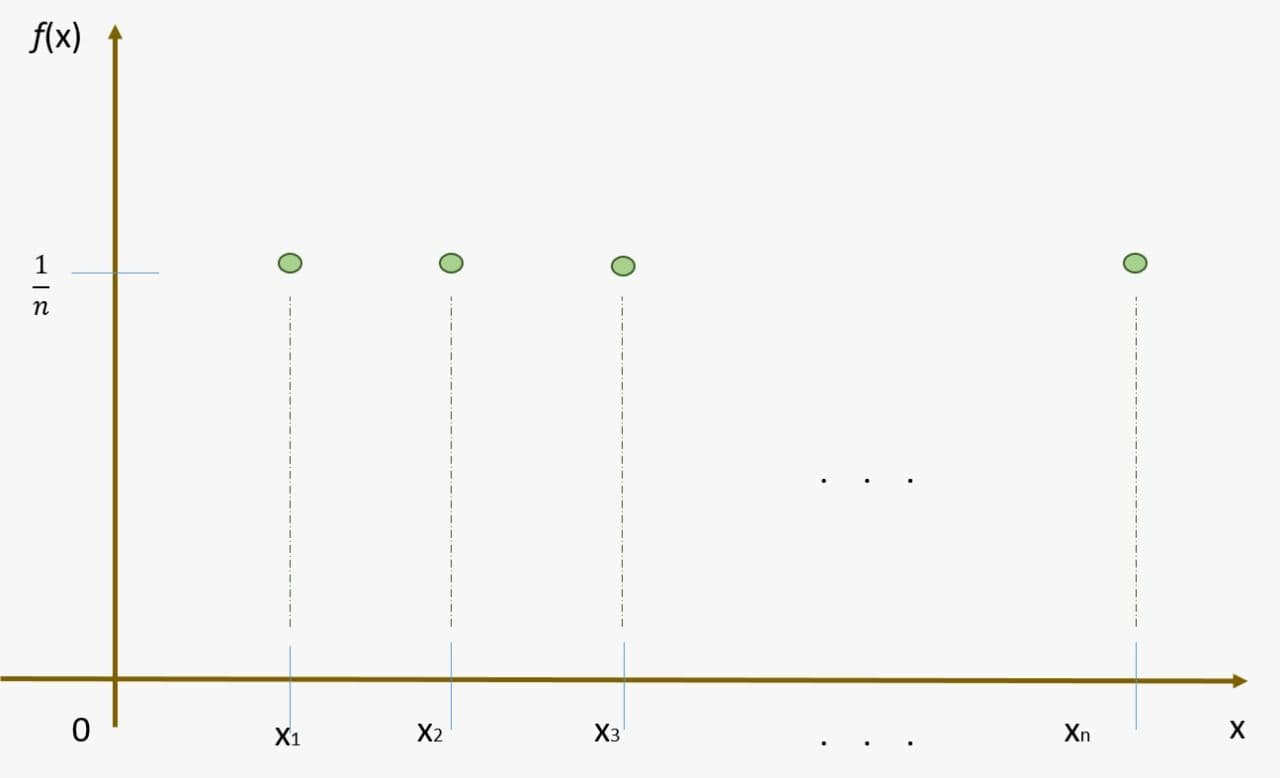
\includegraphics[scale=0.3]{grafica2.jpg}
\end{center}
\begin{center}
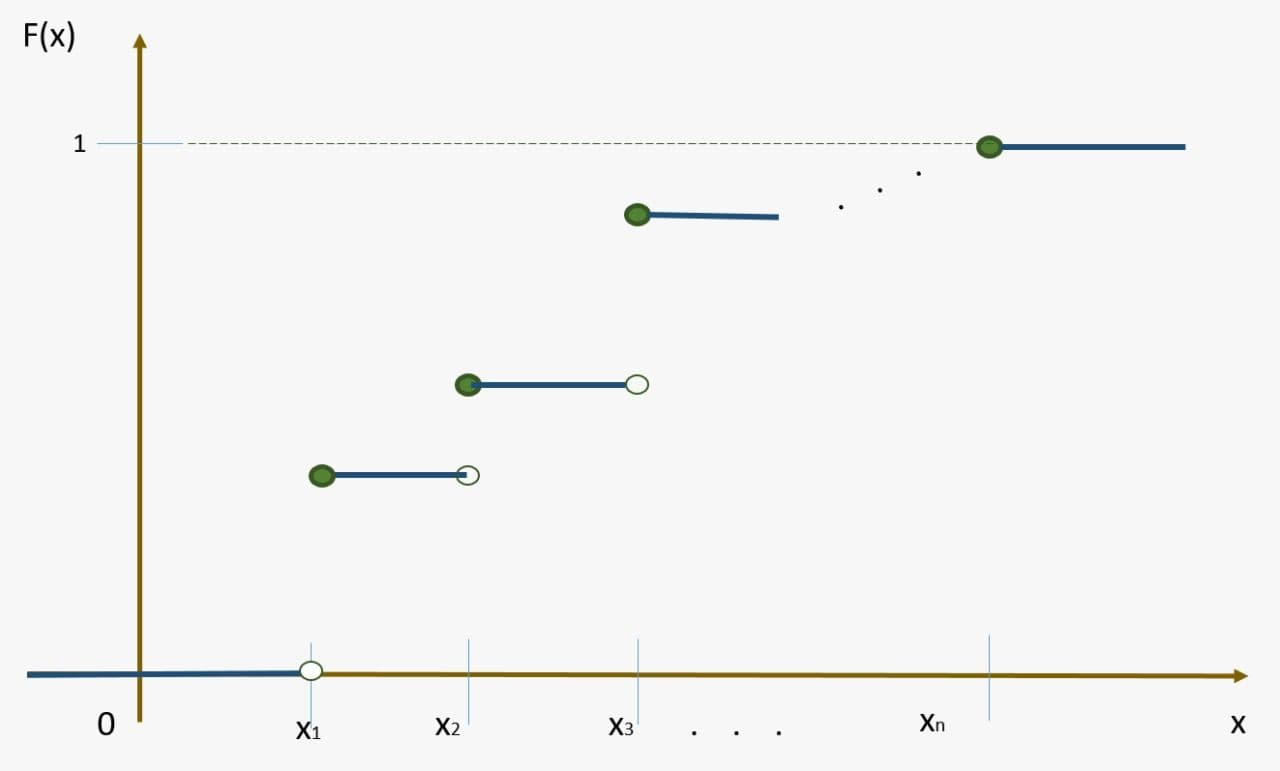
\includegraphics[scale=0.3]{grafica1.jpg}
\end{center}
\section*{Calcular la esperanza matem�tica}
La esperanza de esta distribuci�n puede ser obtenida como una media aritm�tica de los valores que toma la variable $\lbrace  x_{1},x_{2},...,x_{n} \rbrace$.
$$E(x)=\sum_{i=1}^{n}x_{i}f_X(x_{i})=\dfrac{1}{n}\sum_{i=1}^{n}x_{i}=\mu$$
De la misma manera si X es una variable aleatoria  con distribuci�n uniforme discreta en el conjunto $\lbrace 1,...,n \rbrace$. La esperanza cuenta con las siguientes propiedades:\\
A) $E(X) = \dfrac{n + 1}{2}$\\
B) $E(X^2) = \dfrac{(n + 1)(2n + 1)}{6}$
\subsection*{Demostraci�n de la propiedad a)}
Sabemos que:
$$E(x)=\dfrac{1}{n}\sum_{i=1}^{n}x_{i}$$
Conocemos por informaci�n previa que la sumatoria de $\lbrace 1,...,n \rbrace$ puede ser vista como $\dfrac{n(n+1)}{2}$. \\
As� que: 
$$E(X)= \dfrac{1}{n}\sum_{i=1}^{n}x_{i} = \dfrac{1}{n} \cdot \dfrac{n(n+1)}{2} = \dfrac{n + 1}{2}$$
\subsection*{Demostraci�n de la propiedad b)}
Sabemos que:
$$E(x)=\dfrac{1}{n}\sum_{i=1}^{n}x_{i}$$
Conocemos por informaci�n previa que la sumatoria de los cuadrados de $\lbrace 1,...,n \rbrace$ puede ser vista como $\dfrac{n(n+1)(2n+1)}{6}$.\\
As� que:
$$E(X^2)= \dfrac{1}{n}\sum_{i=1}^{n}x^2_{i} = \dfrac{1}{n} \cdot \dfrac{n(n+1)(2n+1)}{6}  = \dfrac{(n + 1)(2n + 1)}{6}$$


\section*{Calcular la varianza}
La varianza se obtiene de la forma ya conocida; es decir, como la varianza de esos mismos valores. Expresada en t�rminos de momentos, la varianza ser�:
$$Var(X)=\dfrac{1}{n}\sum_{i=1}^{n}(x_{i}-\mu)^{2}= \dfrac{1}{n}\sum_{i=1}^{n}(x_{i})^2 - (\mu)^{2} =\sigma ^{2}$$
De igual forma si X es una variable aleatoria  con distribuci�n uniforme discreta en el conjunto $\lbrace 1,...,n \rbrace$. La varianza se puede resumir a:
$$Var(X) = \dfrac{n^{2} + 1}{12}$$
\subsection*{Demostraci�n}
Sabemos que:
$$Var(X)= \dfrac{1}{n}\sum_{i=1}^{n}(x_{i})^2 -(\mu)^{2}$$
Recordando un poco de la ley distributiva de la sumatoria, esto se podr�a ver c�mo:
$$Var(X) =  \dfrac{1}{n}\sum_{i=1}^{n}(x_{i})^2 - \dfrac{1}{n}\sum_{i=1}^{n}(\mu)^{2}$$
Y estose puede ver de la siguiente manera:
$$Var(X) =E(X^2) - E^2(X)$$

Por demostraciones anteriores que realizamos en subtemas atr�s, sabemos que:
$$Var(X) = E(X^2) - E^2(X)= \dfrac{(n + 1)(2n + 1)}{6} - \dfrac{(n +1)^2}{4}$$
$$=\dfrac{8n^2 + 12n + 1 - 6n^2 - 12n - 6}{24}$$
$$= \dfrac{2n^2 - 2}{24}$$
$$= \dfrac{n^2 - 1}{12}$$
\section*{Ejercicios propuestos}
\begin{center}
Supongamos que se lanza una vez un dado. Si el dado est� equilibrado:
\end{center}
a) Defina la funci�n masa de probabilidad.\\
b) Calcule la esperanza.
\subsection*{Soluci�n a)}
Observemos que X es discreta pues $R_{X}= \lbrace 1, 2, 3, 4, 5, 6 \rbrace$. Luego las posibilidades son:

$$f_{X}(1)=P(x=1)=\dfrac{1}{6}$$
$$f_{X}(2)=P(x=2)=\dfrac{1}{6}$$$$f_{X}(3)=P(x=3)=\dfrac{1}{6}$$
$$f_{X}(4)=P(x=4)=\dfrac{1}{6}$$
$$f_{X}(5)=P(x=5)=\dfrac{1}{6}$$
$$f_{X}(6)=P(x=6)=\dfrac{1}{6}$$
 En conclusion:

$$
f_{X} (x)=\begin{cases}
{\dfrac{1}{6}} &\mbox{ $x=1$}\\ 
\\ {\dfrac{1}{6}} &\mbox{$x=2$}\\ 
\\{\dfrac{1}{6}} &\mbox{ $x=3$}\\ 
\\{\dfrac{1}{6}} &\mbox{ $x=4$}\\ 
\\{\dfrac{1}{6}} &\mbox{ $x=5$}\\
\\{\dfrac{1}{6}} &\mbox{$ x=6$}
\end{cases}
$$
\subsection*{Soluci�n b)}
Como la variable aleatoria X tiene distribuci�n uniforme discreta, por defici�n tenemos que:

$$E(x)=\dfrac{1}{n}\sum_{i=1}^{n}x_{i}$$
$$=\dfrac{1}{6}\sum_{i=1}^{6}x_{i}=\dfrac{1}{6}(1+2+3+4+5+6)$$
$$=3.5$$
\end{document}